\clearpage
\subsection{Array} % (fold)
\label{sub:array}

An array is a special kind of \nameref{sub:variable}, one that stores multiple values instead of a single value. The values within an array, called elements, are all of the same \nameref{sub:type}.

\begin{figure}[h]
   \centering
   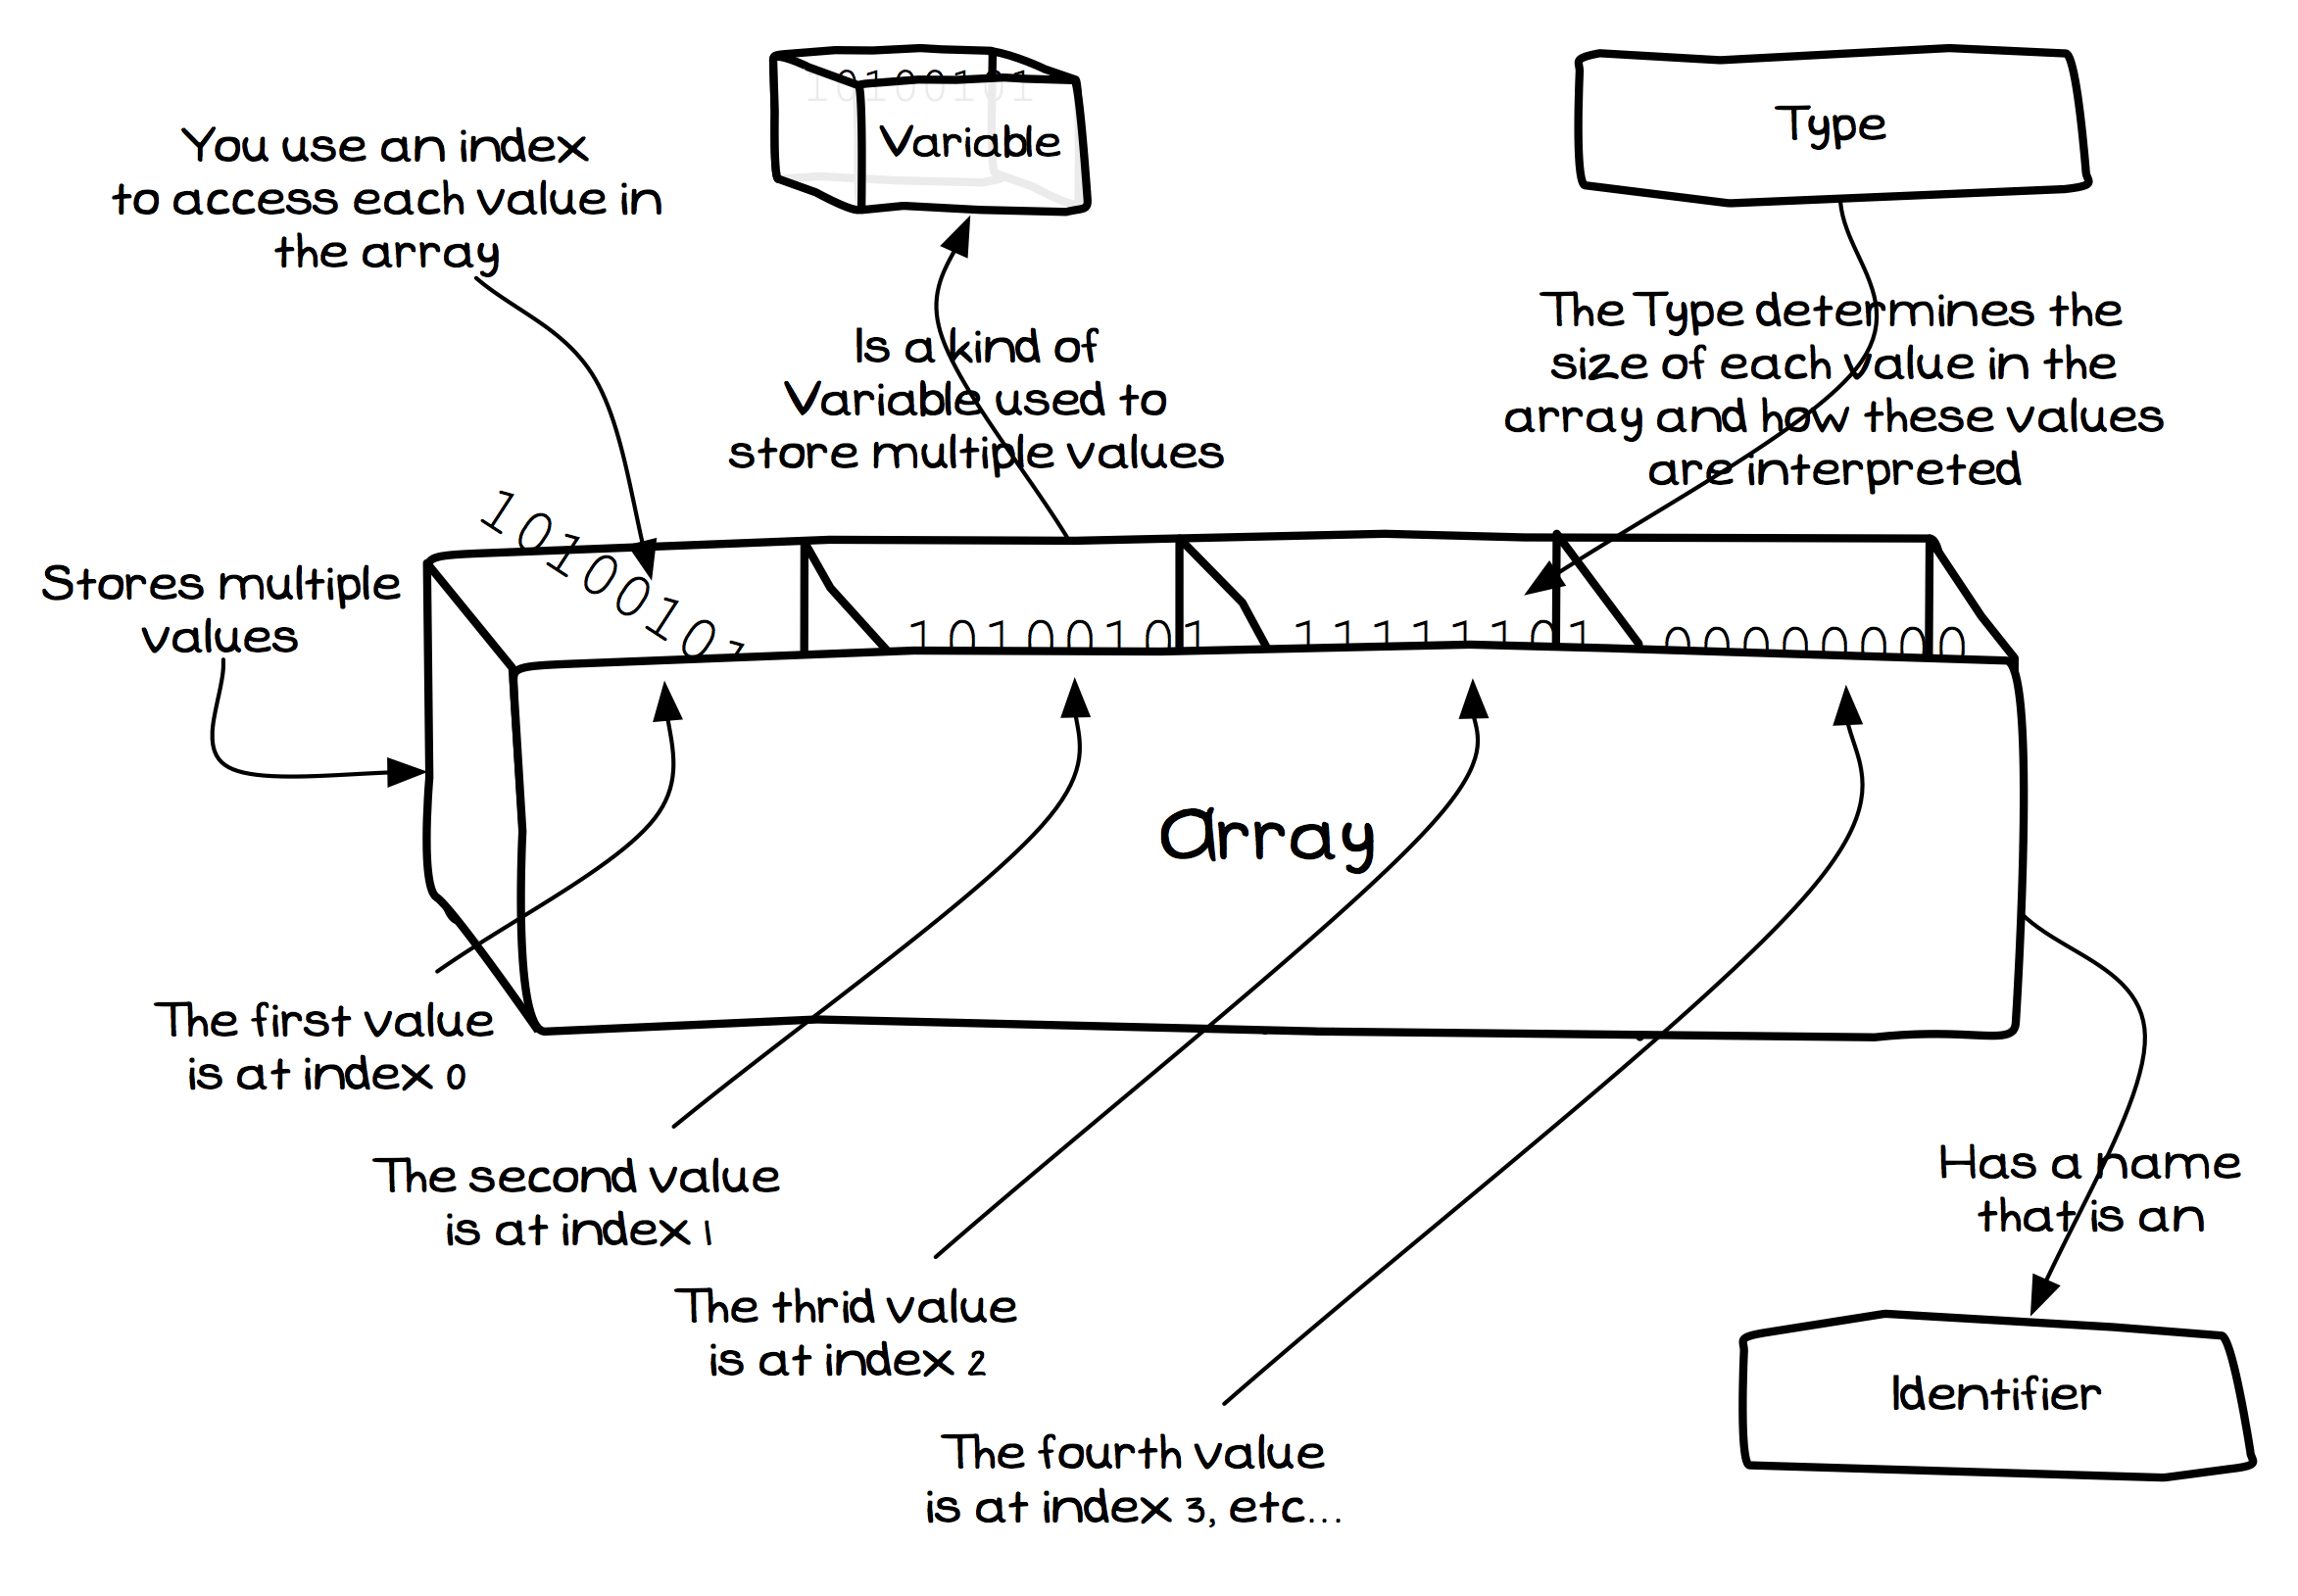
\includegraphics[width=\textwidth]{./topics/arrays/diagrams/Array} 
   \caption{Arrays allow you to store multiple values in a variable}
   \label{fig:type-decl-array}
\end{figure}

\mynote{
\begin{itemize}
  \item An array is an \textbf{artefact}, a kind of variable that you can create in your code.
  \item Each array has a number of elements.
  \item The elements of an array are accessed via an index. The first element has the index~\textbf{0}, the second has the index \textbf{1}, etc. See \nameref{ssub:arrays_in_memory}.
  \item Individual elements of an array are much like a standard variable.
  \item You can store a value in an element of an array using an \nameref{sub:assignment_statement_with_arrays_}.
  \item You can use a the value from an element of an array using \nameref{sub:expressions_with_arrays_}.
  \item The \nameref{sub:for_loop} can be used to perform an action \emph{for each element of an array}.
\end{itemize}
}
\clearpage
\subsubsection{Arrays in Memory} % (fold)
\label{ssub:arrays_in_memory}

Arrays store multiple values, with an index that provides access to the individual elements within the array. Conceptually this can be viewed as a \nameref{sub:variable} that contains multiple slots (the elements) into which the values are stored. 

Many languages have \textbf{0} as the index of the first element. This reflects how the values are actually stored in memory. \fref{fig:type-decl-array-idx} shows how an array (named \texttt{arr} in this Figure) is stored in memory. The array is a \textbf{contiguous} area in memory, with the elements being next to each other. You can think of the array as starting at the first element, so you need to skip \emph{0} elements to access the first element. The second element is accessed by skipping \emph{1} element, so it has index \emph{1}. The third element is accessed by skipping \emph{2} elements, so it has the index \emph{2}, etc.

The size of each of the elements of the array can then be used to quickly locate each element, given its index. If you have an array of \texttt{Integer} values then these are each 32 bits (4 bytes), so the element at index 3 is $3 \times 32bits$ (96 bits) past the start of the array.

The great thing is that you do not need to think about these details, but knowing this should you remember that the first\footnote{Some languages allow you to start at other values, but many use 0 based arrays which map more closely to how the data is stored in memory.} element of an array is at index 0.

\begin{figure}[h]
   \centering
   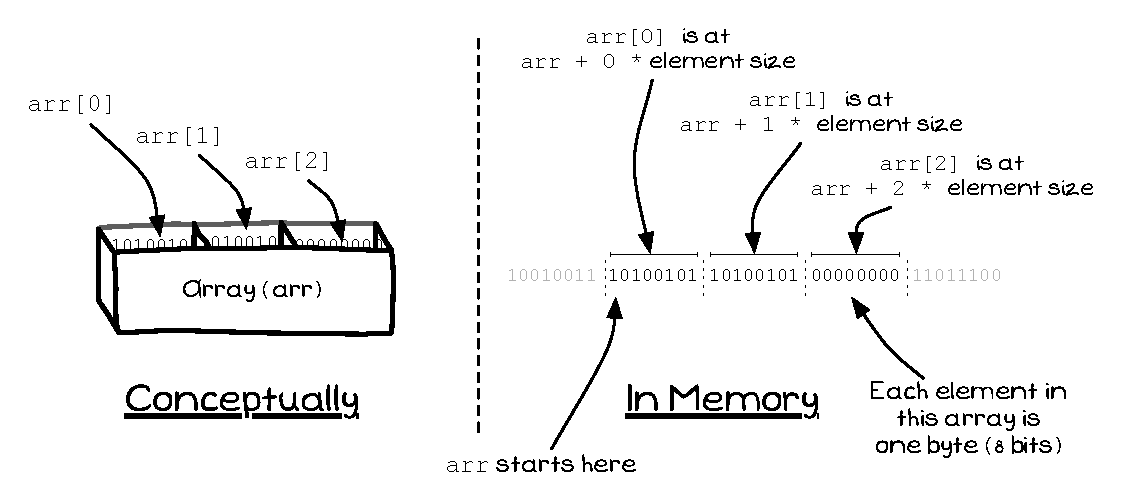
\includegraphics[width=\textwidth]{./topics/arrays/diagrams/ArrayIndex} 
   \caption{Arrays occupy a contiguous area of memory, with elements next to each other in memory }
   \label{fig:type-decl-array-idx}
\end{figure}

\mynote{
\begin{itemize}
  \item Arrays are allocated a contiguous area of memory, with the elements next to each other.
  \item The array index is used to determine how many elements (values) are skipped to access the element you require.
  \item The index of the first element of an array is \textbf{0}.
  \item The last index of the array is therefore \textbf{n - 1}, where \emph{n} is the number of elements in the array.
\end{itemize}
}

% subsubsection arrays_in_memory (end)

% subsection array (end)